% Options for packages loaded elsewhere
\PassOptionsToPackage{unicode}{hyperref}
\PassOptionsToPackage{hyphens}{url}
%
\documentclass[
]{article}
\usepackage{amsmath,amssymb}
\usepackage{iftex}
\ifPDFTeX
  \usepackage[T1]{fontenc}
  \usepackage[utf8]{inputenc}
  \usepackage{textcomp} % provide euro and other symbols
\else % if luatex or xetex
  \usepackage{unicode-math} % this also loads fontspec
  \defaultfontfeatures{Scale=MatchLowercase}
  \defaultfontfeatures[\rmfamily]{Ligatures=TeX,Scale=1}
\fi
\usepackage{lmodern}
\ifPDFTeX\else
  % xetex/luatex font selection
\fi
% Use upquote if available, for straight quotes in verbatim environments
\IfFileExists{upquote.sty}{\usepackage{upquote}}{}
\IfFileExists{microtype.sty}{% use microtype if available
  \usepackage[]{microtype}
  \UseMicrotypeSet[protrusion]{basicmath} % disable protrusion for tt fonts
}{}
\makeatletter
\@ifundefined{KOMAClassName}{% if non-KOMA class
  \IfFileExists{parskip.sty}{%
    \usepackage{parskip}
  }{% else
    \setlength{\parindent}{0pt}
    \setlength{\parskip}{6pt plus 2pt minus 1pt}}
}{% if KOMA class
  \KOMAoptions{parskip=half}}
\makeatother
\usepackage{xcolor}
\usepackage[margin=1in]{geometry}
\usepackage{color}
\usepackage{fancyvrb}
\newcommand{\VerbBar}{|}
\newcommand{\VERB}{\Verb[commandchars=\\\{\}]}
\DefineVerbatimEnvironment{Highlighting}{Verbatim}{commandchars=\\\{\}}
% Add ',fontsize=\small' for more characters per line
\usepackage{framed}
\definecolor{shadecolor}{RGB}{248,248,248}
\newenvironment{Shaded}{\begin{snugshade}}{\end{snugshade}}
\newcommand{\AlertTok}[1]{\textcolor[rgb]{0.94,0.16,0.16}{#1}}
\newcommand{\AnnotationTok}[1]{\textcolor[rgb]{0.56,0.35,0.01}{\textbf{\textit{#1}}}}
\newcommand{\AttributeTok}[1]{\textcolor[rgb]{0.13,0.29,0.53}{#1}}
\newcommand{\BaseNTok}[1]{\textcolor[rgb]{0.00,0.00,0.81}{#1}}
\newcommand{\BuiltInTok}[1]{#1}
\newcommand{\CharTok}[1]{\textcolor[rgb]{0.31,0.60,0.02}{#1}}
\newcommand{\CommentTok}[1]{\textcolor[rgb]{0.56,0.35,0.01}{\textit{#1}}}
\newcommand{\CommentVarTok}[1]{\textcolor[rgb]{0.56,0.35,0.01}{\textbf{\textit{#1}}}}
\newcommand{\ConstantTok}[1]{\textcolor[rgb]{0.56,0.35,0.01}{#1}}
\newcommand{\ControlFlowTok}[1]{\textcolor[rgb]{0.13,0.29,0.53}{\textbf{#1}}}
\newcommand{\DataTypeTok}[1]{\textcolor[rgb]{0.13,0.29,0.53}{#1}}
\newcommand{\DecValTok}[1]{\textcolor[rgb]{0.00,0.00,0.81}{#1}}
\newcommand{\DocumentationTok}[1]{\textcolor[rgb]{0.56,0.35,0.01}{\textbf{\textit{#1}}}}
\newcommand{\ErrorTok}[1]{\textcolor[rgb]{0.64,0.00,0.00}{\textbf{#1}}}
\newcommand{\ExtensionTok}[1]{#1}
\newcommand{\FloatTok}[1]{\textcolor[rgb]{0.00,0.00,0.81}{#1}}
\newcommand{\FunctionTok}[1]{\textcolor[rgb]{0.13,0.29,0.53}{\textbf{#1}}}
\newcommand{\ImportTok}[1]{#1}
\newcommand{\InformationTok}[1]{\textcolor[rgb]{0.56,0.35,0.01}{\textbf{\textit{#1}}}}
\newcommand{\KeywordTok}[1]{\textcolor[rgb]{0.13,0.29,0.53}{\textbf{#1}}}
\newcommand{\NormalTok}[1]{#1}
\newcommand{\OperatorTok}[1]{\textcolor[rgb]{0.81,0.36,0.00}{\textbf{#1}}}
\newcommand{\OtherTok}[1]{\textcolor[rgb]{0.56,0.35,0.01}{#1}}
\newcommand{\PreprocessorTok}[1]{\textcolor[rgb]{0.56,0.35,0.01}{\textit{#1}}}
\newcommand{\RegionMarkerTok}[1]{#1}
\newcommand{\SpecialCharTok}[1]{\textcolor[rgb]{0.81,0.36,0.00}{\textbf{#1}}}
\newcommand{\SpecialStringTok}[1]{\textcolor[rgb]{0.31,0.60,0.02}{#1}}
\newcommand{\StringTok}[1]{\textcolor[rgb]{0.31,0.60,0.02}{#1}}
\newcommand{\VariableTok}[1]{\textcolor[rgb]{0.00,0.00,0.00}{#1}}
\newcommand{\VerbatimStringTok}[1]{\textcolor[rgb]{0.31,0.60,0.02}{#1}}
\newcommand{\WarningTok}[1]{\textcolor[rgb]{0.56,0.35,0.01}{\textbf{\textit{#1}}}}
\usepackage{longtable,booktabs,array}
\usepackage{calc} % for calculating minipage widths
% Correct order of tables after \paragraph or \subparagraph
\usepackage{etoolbox}
\makeatletter
\patchcmd\longtable{\par}{\if@noskipsec\mbox{}\fi\par}{}{}
\makeatother
% Allow footnotes in longtable head/foot
\IfFileExists{footnotehyper.sty}{\usepackage{footnotehyper}}{\usepackage{footnote}}
\makesavenoteenv{longtable}
\usepackage{graphicx}
\makeatletter
\def\maxwidth{\ifdim\Gin@nat@width>\linewidth\linewidth\else\Gin@nat@width\fi}
\def\maxheight{\ifdim\Gin@nat@height>\textheight\textheight\else\Gin@nat@height\fi}
\makeatother
% Scale images if necessary, so that they will not overflow the page
% margins by default, and it is still possible to overwrite the defaults
% using explicit options in \includegraphics[width, height, ...]{}
\setkeys{Gin}{width=\maxwidth,height=\maxheight,keepaspectratio}
% Set default figure placement to htbp
\makeatletter
\def\fps@figure{htbp}
\makeatother
\setlength{\emergencystretch}{3em} % prevent overfull lines
\providecommand{\tightlist}{%
  \setlength{\itemsep}{0pt}\setlength{\parskip}{0pt}}
\setcounter{secnumdepth}{-\maxdimen} % remove section numbering
\ifLuaTeX
  \usepackage{selnolig}  % disable illegal ligatures
\fi
\usepackage{bookmark}
\IfFileExists{xurl.sty}{\usepackage{xurl}}{} % add URL line breaks if available
\urlstyle{same}
\hypersetup{
  pdftitle={VonBEE: State-space vonB growth model with environmental covariates},
  pdfauthor={K. K. Holsman, J. Ianelli, et al.},
  hidelinks,
  pdfcreator={LaTeX via pandoc}}

\title{VonBEE: State-space vonB growth model with environmental
covariates}
\author{K. K. Holsman, J. Ianelli, et al.}
\date{}

\begin{document}
\maketitle

{
\setcounter{tocdepth}{2}
\tableofcontents
}

\includegraphics[width=0.25\textwidth,height=\textheight]{Figs/vonBEE.png}

Last updated: Oct 04, 2024\\
github repo: \url{https://github.com/kholsman/vonBEE}\\
\url{https://noaa-reem.github.io/vonBEE/}

\section{Install the package vonBEE}\label{install-the-package-vonbee}

\begin{Shaded}
\begin{Highlighting}[]
\NormalTok{  missing }\OtherTok{\textless{}{-}} \FunctionTok{setdiff}\NormalTok{(}\FunctionTok{c}\NormalTok{(}\StringTok{"devtools"}\NormalTok{,}\StringTok{"usethis"}\NormalTok{),   }\FunctionTok{installed.packages}\NormalTok{()[, }\DecValTok{1}\NormalTok{])}
  \ControlFlowTok{if}\NormalTok{ (}\FunctionTok{length}\NormalTok{(missing) }\SpecialCharTok{\textgreater{}} \DecValTok{0}\NormalTok{)  }\FunctionTok{install.packages}\NormalTok{(missing)}

\NormalTok{  devtools}\SpecialCharTok{::}\FunctionTok{install\_github}\NormalTok{(}\StringTok{"NOAA{-}REEM/vonBEE"}\NormalTok{)}
\end{Highlighting}
\end{Shaded}

\section{Introduction}\label{introduction}

\begin{itemize}
\tightlist
\item[$\square$]
  Add intro paragraph about climate effects on growth
\end{itemize}

Water temperature is known to directly impact growth through influencing
metabolic and digestion rates, which often scale exponentially with body
weight and temperature (see Hanson et al., 1997 for an overview).

(based on \url{https://seananderson.ca/2014/10/17/tmb/})

\section{Methods}\label{methods}

\subsection{Temperature specific weight at
age}\label{temperature-specific-weight-at-age}

We modified the generalized formulation of the von Bertalanffy growth
function (VBGF; von Bertalanffy 1938; Pauly 1981; Temming 1994) to
predict temperature-dependent growth by allowing the allometric scaling
parameter \(d\) to increase with temperature. Essington et al.~(2010)
and Holsman and Aydin (2015), and Holsman et al.~(2016) describe the
derivation and application of the VBGF towards bioenergetics modeling in
great detail, so we do not repeat it here. Essentially, in this
formulation \(d\) represents the realized allometric slope of
consumption, which integrates both the direct effect of temperature on
consumption and indirect ecological interactions that scale with
temperature and influence relative foraging rates (see Essington et al.,
2010; Holsman and Aydin, 2015). We fit the VBGF to otolith-based length-
and weight-at-age data (\(n\) = 21,388, 14,362, and 772, for pollock,
Pacific cod, and arrowtooth flounder, respectively) collected during
AFSC Bering Sea surveys and analyzed at the AFSC (REF).

For each species, we used the vonBT() model to fit a state-space
environmental growth model for fish weight and age data using the base
state-space model (based on Gompertz et al.~20XX):

Eq. 1
\[ ln(\hat{W}{i}) = W^\infty{i} + \frac{1}{(1-d_{i})}log(1-e^{-K(1-d_{i})(A_i-t_0)})+\varepsilon_i\sim N(0,\sigma^2{obs})\]
, where

Eq. 2 \[W^\infty_{i} =(\frac{H}{K})^{\frac{1}{(1 - d_{i})}} \]

where \(t_{0,i}\) is the age at which \(W_{i} = 0\), \(W^{\infty}_{i}\)
is the asymptotic mass which can vary by individual \(i\) cohort year
effects, \(H\) is the assimilation constant \(K\) is the energy loss
constant (Essington et al., 2010), and \(\varepsilon_i\) is a normally
and independently distributed random variable with mean 0 and variance
\(\sigma_{obs}^2\). Essington et al.~(2010) and Holsman and Aydin,
(2015) statistically estimated the \(d\), \(K\) and \(H\) parameters for
various species to estimate consumption rates. In particular, Holsman
and Aydin (2015) found that the \(d\) parameter varied between species
and regions in Alaska (USA). We further modified this approach to
estimate the environment impacts growth on growth annually for each year
\(y\) through a logistic model that includes a vector of annual
covariates (\(X_{c,y}\)) effects on \(d\) (which ranges between 0 and
1). where \(\alpha0_{d,i}\) and \(\alpha_{d,i,y}\) represent the mean
the \(d\) consumption parameter intercept and \(\beta_{c}\) is the
coefficient for the residual effect of an environmental variable on the
\(d\) consumption parameter, such that:

Eq. 3
\[d_{i} = 1/(1+e^{-(U_{y}+\beta_{0,y_{y-A_i}}+\sum_c(\beta_{c}*X_{c,y})}) \]

We chose this formulation based on the empirical relationship between
temperature and consumption, assuming that \(d\) would capture the
differential effects of temperature on growth, and that waste rates
scale proportionally with weight but do not vary over time with diet or
temperature (i.e.~\(K\) is constant but \(d\) can vary with
temperature). This formulation allows both the slope and asymptotic
limit of growth to vary with temperature. Similar approaches, with
slightly different modifications to the VBGF, including temperature and
prey specific terms for \(d\) and \(K\), respectively, have been used
elsewhere to evaluate climate impacts on fish growth (e.g., Cheung et
al., 2015; Hamre, 2003).

We further modeled the \(d\) consumption parameter as a state-space
model that estimates random effects on \(U_{y}\) as the unobserved state
vector:

Eq. 4 \[ U_{y} = \mu+ \beta_{1}U_{y-1}+\varepsilon_y \] Process error is
then modeled as a normal distribution with mean of 0 and standard
deviation of \(\sigma_{proc}\):

Eq. 5 \[ \varepsilon_{y} \sim N(0,\sigma^2_{proc})\]

Optionally, there can be auto regressive (state-space) terms included as
\(\beta_1\) (e.g., if growth the previous year impacts growth in
observation year). Cohort year (\(Y_{y-A_i}\) ) effects can also be
included as random or fixed effects via \(\beta_{0,y_{y-A_i}}\). If
these terms are not included the model simplifies to a random (process
error) annual intercept ( \(\mu\)) plus covariate effects. If covariate
terms are further not included and the random process error is not
estimated the model simplifies to the generalized VonB.

Weight at age is then modeled as:

Eq. 6 \[ ln({W}_i) \sim N(ln(\hat{W}_i),\sigma^2_{obs})\] where
\(\sigma_{obs}\) is the standard deviation of observation error (log
scale).

\section{Results}\label{results}

Comparative model fits using average observed bottom temperature are
included below.

\begin{itemize}
\tightlist
\item[$\square$]
  Next add in G potential from energetic indices as a covariate.
\end{itemize}

\subsection{Eastern Bering Sea}\label{eastern-bering-sea}

\subsubsection{EBS pollock}\label{ebs-pollock}

\begin{figure}

{\centering \includegraphics[width=1\linewidth]{data/out/BS/walleye pollock/Figs/model_plots} 

}

\caption{Comparative model fits to observed weight at age data}\label{fig:unnamed-chunk-2}
\end{figure}

\begin{figure}

{\centering \includegraphics[width=1\linewidth]{data/out/BS/walleye pollock/Figs/model_Temp_byage2} 

}

\caption{Temperature effects on weight at age}\label{fig:unnamed-chunk-3}
\end{figure}

\begin{longtable}[]{@{}
  >{\raggedright\arraybackslash}p{(\columnwidth - 16\tabcolsep) * \real{0.1061}}
  >{\raggedright\arraybackslash}p{(\columnwidth - 16\tabcolsep) * \real{0.1212}}
  >{\raggedleft\arraybackslash}p{(\columnwidth - 16\tabcolsep) * \real{0.0758}}
  >{\raggedleft\arraybackslash}p{(\columnwidth - 16\tabcolsep) * \real{0.1364}}
  >{\raggedleft\arraybackslash}p{(\columnwidth - 16\tabcolsep) * \real{0.0455}}
  >{\raggedleft\arraybackslash}p{(\columnwidth - 16\tabcolsep) * \real{0.0909}}
  >{\raggedleft\arraybackslash}p{(\columnwidth - 16\tabcolsep) * \real{0.1515}}
  >{\raggedleft\arraybackslash}p{(\columnwidth - 16\tabcolsep) * \real{0.1061}}
  >{\raggedleft\arraybackslash}p{(\columnwidth - 16\tabcolsep) * \real{0.1667}}@{}}
\caption{AIcc results for BS walleye pollock}\tabularnewline
\toprule\noalign{}
\begin{minipage}[b]{\linewidth}\raggedright
model
\end{minipage} & \begin{minipage}[b]{\linewidth}\raggedright
top\_set
\end{minipage} & \begin{minipage}[b]{\linewidth}\raggedleft
r2
\end{minipage} & \begin{minipage}[b]{\linewidth}\raggedleft
nll
\end{minipage} & \begin{minipage}[b]{\linewidth}\raggedleft
k
\end{minipage} & \begin{minipage}[b]{\linewidth}\raggedleft
n
\end{minipage} & \begin{minipage}[b]{\linewidth}\raggedleft
delta\_aic
\end{minipage} & \begin{minipage}[b]{\linewidth}\raggedleft
aic\_wt
\end{minipage} & \begin{minipage}[b]{\linewidth}\raggedleft
sum\_aic\_wt
\end{minipage} \\
\midrule\noalign{}
\endfirsthead
\toprule\noalign{}
\begin{minipage}[b]{\linewidth}\raggedright
model
\end{minipage} & \begin{minipage}[b]{\linewidth}\raggedright
top\_set
\end{minipage} & \begin{minipage}[b]{\linewidth}\raggedleft
r2
\end{minipage} & \begin{minipage}[b]{\linewidth}\raggedleft
nll
\end{minipage} & \begin{minipage}[b]{\linewidth}\raggedleft
k
\end{minipage} & \begin{minipage}[b]{\linewidth}\raggedleft
n
\end{minipage} & \begin{minipage}[b]{\linewidth}\raggedleft
delta\_aic
\end{minipage} & \begin{minipage}[b]{\linewidth}\raggedleft
aic\_wt
\end{minipage} & \begin{minipage}[b]{\linewidth}\raggedleft
sum\_aic\_wt
\end{minipage} \\
\midrule\noalign{}
\endhead
\bottomrule\noalign{}
\endlastfoot
m5 & TRUE & 0.80 & 14791.21 & 11 & 35617 & 0.00 & 1 & 1 \\
m2 & FALSE & 0.77 & 16070.69 & 9 & 35617 & 2554.96 & 0 & 1 \\
m0 & FALSE & 0.77 & 16206.30 & 5 & 35617 & 2818.16 & 0 & 1 \\
m1 & NA & 0.77 & 16070.79 & 7 & 35617 & NA & NA & NA \\
m3 & NA & 0.78 & 15699.80 & 58 & 35617 & NA & NA & NA \\
m3\_rnd & NA & 0.78 & 15891.81 & 9 & 35617 & NA & NA & NA \\
m4 & NA & 0.79 & 15400.81 & 11 & 35617 & NA & NA & NA \\
\end{longtable}

\subsubsection{EBS Pacific cod}\label{ebs-pacific-cod}

\begin{figure}

{\centering \includegraphics[width=1\linewidth]{data/out/BS/Pacific cod/Figs/model_plots} 

}

\caption{Comparative model fits to observed weight at age data}\label{fig:unnamed-chunk-6}
\end{figure}

\begin{figure}

{\centering \includegraphics[width=1\linewidth]{data/out/BS/Pacific cod/Figs/model_Temp_byage2} 

}

\caption{Temperature effects on weight at age}\label{fig:unnamed-chunk-7}
\end{figure}

\begin{longtable}[]{@{}
  >{\raggedright\arraybackslash}p{(\columnwidth - 16\tabcolsep) * \real{0.1061}}
  >{\raggedright\arraybackslash}p{(\columnwidth - 16\tabcolsep) * \real{0.1212}}
  >{\raggedleft\arraybackslash}p{(\columnwidth - 16\tabcolsep) * \real{0.0758}}
  >{\raggedleft\arraybackslash}p{(\columnwidth - 16\tabcolsep) * \real{0.1364}}
  >{\raggedleft\arraybackslash}p{(\columnwidth - 16\tabcolsep) * \real{0.0455}}
  >{\raggedleft\arraybackslash}p{(\columnwidth - 16\tabcolsep) * \real{0.0909}}
  >{\raggedleft\arraybackslash}p{(\columnwidth - 16\tabcolsep) * \real{0.1515}}
  >{\raggedleft\arraybackslash}p{(\columnwidth - 16\tabcolsep) * \real{0.1061}}
  >{\raggedleft\arraybackslash}p{(\columnwidth - 16\tabcolsep) * \real{0.1667}}@{}}
\caption{AIcc results for BS Pacific cod}\tabularnewline
\toprule\noalign{}
\begin{minipage}[b]{\linewidth}\raggedright
model
\end{minipage} & \begin{minipage}[b]{\linewidth}\raggedright
top\_set
\end{minipage} & \begin{minipage}[b]{\linewidth}\raggedleft
r2
\end{minipage} & \begin{minipage}[b]{\linewidth}\raggedleft
nll
\end{minipage} & \begin{minipage}[b]{\linewidth}\raggedleft
k
\end{minipage} & \begin{minipage}[b]{\linewidth}\raggedleft
n
\end{minipage} & \begin{minipage}[b]{\linewidth}\raggedleft
delta\_aic
\end{minipage} & \begin{minipage}[b]{\linewidth}\raggedleft
aic\_wt
\end{minipage} & \begin{minipage}[b]{\linewidth}\raggedleft
sum\_aic\_wt
\end{minipage} \\
\midrule\noalign{}
\endfirsthead
\toprule\noalign{}
\begin{minipage}[b]{\linewidth}\raggedright
model
\end{minipage} & \begin{minipage}[b]{\linewidth}\raggedright
top\_set
\end{minipage} & \begin{minipage}[b]{\linewidth}\raggedleft
r2
\end{minipage} & \begin{minipage}[b]{\linewidth}\raggedleft
nll
\end{minipage} & \begin{minipage}[b]{\linewidth}\raggedleft
k
\end{minipage} & \begin{minipage}[b]{\linewidth}\raggedleft
n
\end{minipage} & \begin{minipage}[b]{\linewidth}\raggedleft
delta\_aic
\end{minipage} & \begin{minipage}[b]{\linewidth}\raggedleft
aic\_wt
\end{minipage} & \begin{minipage}[b]{\linewidth}\raggedleft
sum\_aic\_wt
\end{minipage} \\
\midrule\noalign{}
\endhead
\bottomrule\noalign{}
\endlastfoot
m4 & TRUE & 0.76 & 17174.24 & 11 & 28034 & 0.00 & 1 & 1 \\
m2 & FALSE & 0.78 & 18463.98 & 9 & 28034 & 2575.48 & 0 & 1 \\
m1 & FALSE & 0.77 & 18771.32 & 7 & 28034 & 3186.15 & 0 & 1 \\
m0 & FALSE & 0.78 & 19240.30 & 5 & 28034 & 4120.12 & 0 & 1 \\
m3 & NA & 0.78 & 16959.47 & 51 & 28034 & NA & NA & NA \\
m3\_rnd & NA & 0.78 & 17010.33 & 9 & 28034 & NA & NA & NA \\
m5 & NA & 0.77 & 16491.97 & 11 & 28034 & NA & NA & NA \\
\end{longtable}

\subsubsection{EBS arrowtooth flounder}\label{ebs-arrowtooth-flounder}

\begin{figure}

{\centering \includegraphics[width=1\linewidth]{data/out/BS/arrowtooth flounder/Figs/model_plots} 

}

\caption{Comparative model fits to observed weight at age data}\label{fig:unnamed-chunk-10}
\end{figure}

\begin{figure}

{\centering \includegraphics[width=1\linewidth]{data/out/BS/arrowtooth flounder/Figs/model_Temp_byage2} 

}

\caption{Temperature effects on weight at age}\label{fig:unnamed-chunk-11}
\end{figure}

\begin{longtable}[]{@{}
  >{\raggedright\arraybackslash}p{(\columnwidth - 16\tabcolsep) * \real{0.1077}}
  >{\raggedright\arraybackslash}p{(\columnwidth - 16\tabcolsep) * \real{0.1231}}
  >{\raggedleft\arraybackslash}p{(\columnwidth - 16\tabcolsep) * \real{0.0769}}
  >{\raggedleft\arraybackslash}p{(\columnwidth - 16\tabcolsep) * \real{0.1385}}
  >{\raggedleft\arraybackslash}p{(\columnwidth - 16\tabcolsep) * \real{0.0462}}
  >{\raggedleft\arraybackslash}p{(\columnwidth - 16\tabcolsep) * \real{0.0769}}
  >{\raggedleft\arraybackslash}p{(\columnwidth - 16\tabcolsep) * \real{0.1538}}
  >{\raggedleft\arraybackslash}p{(\columnwidth - 16\tabcolsep) * \real{0.1077}}
  >{\raggedleft\arraybackslash}p{(\columnwidth - 16\tabcolsep) * \real{0.1692}}@{}}
\caption{AIcc results for BS arrowtooth flounder}\tabularnewline
\toprule\noalign{}
\begin{minipage}[b]{\linewidth}\raggedright
model
\end{minipage} & \begin{minipage}[b]{\linewidth}\raggedright
top\_set
\end{minipage} & \begin{minipage}[b]{\linewidth}\raggedleft
r2
\end{minipage} & \begin{minipage}[b]{\linewidth}\raggedleft
nll
\end{minipage} & \begin{minipage}[b]{\linewidth}\raggedleft
k
\end{minipage} & \begin{minipage}[b]{\linewidth}\raggedleft
n
\end{minipage} & \begin{minipage}[b]{\linewidth}\raggedleft
delta\_aic
\end{minipage} & \begin{minipage}[b]{\linewidth}\raggedleft
aic\_wt
\end{minipage} & \begin{minipage}[b]{\linewidth}\raggedleft
sum\_aic\_wt
\end{minipage} \\
\midrule\noalign{}
\endfirsthead
\toprule\noalign{}
\begin{minipage}[b]{\linewidth}\raggedright
model
\end{minipage} & \begin{minipage}[b]{\linewidth}\raggedright
top\_set
\end{minipage} & \begin{minipage}[b]{\linewidth}\raggedleft
r2
\end{minipage} & \begin{minipage}[b]{\linewidth}\raggedleft
nll
\end{minipage} & \begin{minipage}[b]{\linewidth}\raggedleft
k
\end{minipage} & \begin{minipage}[b]{\linewidth}\raggedleft
n
\end{minipage} & \begin{minipage}[b]{\linewidth}\raggedleft
delta\_aic
\end{minipage} & \begin{minipage}[b]{\linewidth}\raggedleft
aic\_wt
\end{minipage} & \begin{minipage}[b]{\linewidth}\raggedleft
sum\_aic\_wt
\end{minipage} \\
\midrule\noalign{}
\endhead
\bottomrule\noalign{}
\endlastfoot
m2 & TRUE & 0.77 & 3153.059 & 9 & 6467 & 0.00 & 1 & 1 \\
m1 & FALSE & 0.76 & 3218.419 & 7 & 6467 & 126.71 & 0 & 1 \\
m0 & FALSE & 0.76 & 3344.602 & 5 & 6467 & 375.07 & 0 & 1 \\
m3 & NA & 0.77 & 3039.064 & 46 & 6467 & NA & NA & NA \\
m3\_rnd & NA & 0.77 & 3167.428 & 9 & 6467 & NA & NA & NA \\
m4 & NA & 0.76 & 3111.604 & 11 & 6467 & NA & NA & NA \\
m5 & NA & 0.77 & 3073.734 & 11 & 6467 & NA & NA & NA \\
\end{longtable}

\subsubsection{EBS sablefish}\label{ebs-sablefish}

\subsubsection{EBS yellowfin sole}\label{ebs-yellowfin-sole}

\begin{figure}

{\centering \includegraphics[width=1\linewidth]{data/out/BS/yellowfin sole/Figs/model_plots} 

}

\caption{Comparative model fits to observed weight at age data}\label{fig:unnamed-chunk-14}
\end{figure}

\begin{figure}

{\centering \includegraphics[width=1\linewidth]{data/out/BS/yellowfin sole/Figs/model_Temp_byage2} 

}

\caption{Temperature effects on weight at age}\label{fig:unnamed-chunk-15}
\end{figure}

\begin{longtable}[]{@{}
  >{\raggedright\arraybackslash}p{(\columnwidth - 16\tabcolsep) * \real{0.0811}}
  >{\raggedright\arraybackslash}p{(\columnwidth - 16\tabcolsep) * \real{0.1081}}
  >{\raggedleft\arraybackslash}p{(\columnwidth - 16\tabcolsep) * \real{0.0676}}
  >{\raggedleft\arraybackslash}p{(\columnwidth - 16\tabcolsep) * \real{0.1351}}
  >{\raggedleft\arraybackslash}p{(\columnwidth - 16\tabcolsep) * \real{0.0405}}
  >{\raggedleft\arraybackslash}p{(\columnwidth - 16\tabcolsep) * \real{0.1892}}
  >{\raggedleft\arraybackslash}p{(\columnwidth - 16\tabcolsep) * \real{0.1351}}
  >{\raggedleft\arraybackslash}p{(\columnwidth - 16\tabcolsep) * \real{0.0946}}
  >{\raggedleft\arraybackslash}p{(\columnwidth - 16\tabcolsep) * \real{0.1486}}@{}}
\caption{AIcc results for BS yellowfin sole}\tabularnewline
\toprule\noalign{}
\begin{minipage}[b]{\linewidth}\raggedright
model
\end{minipage} & \begin{minipage}[b]{\linewidth}\raggedright
top\_set
\end{minipage} & \begin{minipage}[b]{\linewidth}\raggedleft
r2
\end{minipage} & \begin{minipage}[b]{\linewidth}\raggedleft
nll
\end{minipage} & \begin{minipage}[b]{\linewidth}\raggedleft
k
\end{minipage} & \begin{minipage}[b]{\linewidth}\raggedleft
n
\end{minipage} & \begin{minipage}[b]{\linewidth}\raggedleft
delta\_aic
\end{minipage} & \begin{minipage}[b]{\linewidth}\raggedleft
aic\_wt
\end{minipage} & \begin{minipage}[b]{\linewidth}\raggedleft
sum\_aic\_wt
\end{minipage} \\
\midrule\noalign{}
\endfirsthead
\toprule\noalign{}
\begin{minipage}[b]{\linewidth}\raggedright
model
\end{minipage} & \begin{minipage}[b]{\linewidth}\raggedright
top\_set
\end{minipage} & \begin{minipage}[b]{\linewidth}\raggedleft
r2
\end{minipage} & \begin{minipage}[b]{\linewidth}\raggedleft
nll
\end{minipage} & \begin{minipage}[b]{\linewidth}\raggedleft
k
\end{minipage} & \begin{minipage}[b]{\linewidth}\raggedleft
n
\end{minipage} & \begin{minipage}[b]{\linewidth}\raggedleft
delta\_aic
\end{minipage} & \begin{minipage}[b]{\linewidth}\raggedleft
aic\_wt
\end{minipage} & \begin{minipage}[b]{\linewidth}\raggedleft
sum\_aic\_wt
\end{minipage} \\
\midrule\noalign{}
\endhead
\bottomrule\noalign{}
\endlastfoot
m4 & TRUE & 0.76 & 8935.907 & 11 & -0.8866068 & 0.00 & 1 & 1 \\
m2 & FALSE & 0.76 & 9136.776 & 9 & 16739.0000000 & 418.24 & 0 & 1 \\
m1 & FALSE & 0.76 & 9347.177 & 7 & 16739.0000000 & 835.03 & 0 & 1 \\
m0 & FALSE & 0.76 & 9358.274 & 5 & 16739.0000000 & 853.22 & 0 & 1 \\
m3 & FALSE & 0.69 & 13307.331 & 66 & 16739.0000000 & 8873.87 & 0 & 1 \\
\end{longtable}

\subsection{Gulf of Alaska}\label{gulf-of-alaska}

\subsubsection{EBS pollock}\label{ebs-pollock-1}

\begin{figure}

{\centering \includegraphics[width=1\linewidth]{data/out/GOA/walleye pollock/Figs/model_plots} 

}

\caption{Comparative model fits to observed weight at age data}\label{fig:unnamed-chunk-18}
\end{figure}

\begin{figure}

{\centering \includegraphics[width=1\linewidth]{data/out/GOA/walleye pollock/Figs/model_Temp_byage2} 

}

\caption{Temperature effects on weight at age}\label{fig:unnamed-chunk-19}
\end{figure}

\begin{longtable}[]{@{}
  >{\raggedright\arraybackslash}p{(\columnwidth - 16\tabcolsep) * \real{0.0946}}
  >{\raggedright\arraybackslash}p{(\columnwidth - 16\tabcolsep) * \real{0.1081}}
  >{\raggedleft\arraybackslash}p{(\columnwidth - 16\tabcolsep) * \real{0.0676}}
  >{\raggedleft\arraybackslash}p{(\columnwidth - 16\tabcolsep) * \real{0.1216}}
  >{\raggedleft\arraybackslash}p{(\columnwidth - 16\tabcolsep) * \real{0.0405}}
  >{\raggedleft\arraybackslash}p{(\columnwidth - 16\tabcolsep) * \real{0.1892}}
  >{\raggedleft\arraybackslash}p{(\columnwidth - 16\tabcolsep) * \real{0.1351}}
  >{\raggedleft\arraybackslash}p{(\columnwidth - 16\tabcolsep) * \real{0.0946}}
  >{\raggedleft\arraybackslash}p{(\columnwidth - 16\tabcolsep) * \real{0.1486}}@{}}
\caption{AIcc results for GOA walleye pollock}\tabularnewline
\toprule\noalign{}
\begin{minipage}[b]{\linewidth}\raggedright
model
\end{minipage} & \begin{minipage}[b]{\linewidth}\raggedright
top\_set
\end{minipage} & \begin{minipage}[b]{\linewidth}\raggedleft
r2
\end{minipage} & \begin{minipage}[b]{\linewidth}\raggedleft
nll
\end{minipage} & \begin{minipage}[b]{\linewidth}\raggedleft
k
\end{minipage} & \begin{minipage}[b]{\linewidth}\raggedleft
n
\end{minipage} & \begin{minipage}[b]{\linewidth}\raggedleft
delta\_aic
\end{minipage} & \begin{minipage}[b]{\linewidth}\raggedleft
aic\_wt
\end{minipage} & \begin{minipage}[b]{\linewidth}\raggedleft
sum\_aic\_wt
\end{minipage} \\
\midrule\noalign{}
\endfirsthead
\toprule\noalign{}
\begin{minipage}[b]{\linewidth}\raggedright
model
\end{minipage} & \begin{minipage}[b]{\linewidth}\raggedright
top\_set
\end{minipage} & \begin{minipage}[b]{\linewidth}\raggedleft
r2
\end{minipage} & \begin{minipage}[b]{\linewidth}\raggedleft
nll
\end{minipage} & \begin{minipage}[b]{\linewidth}\raggedleft
k
\end{minipage} & \begin{minipage}[b]{\linewidth}\raggedleft
n
\end{minipage} & \begin{minipage}[b]{\linewidth}\raggedleft
delta\_aic
\end{minipage} & \begin{minipage}[b]{\linewidth}\raggedleft
aic\_wt
\end{minipage} & \begin{minipage}[b]{\linewidth}\raggedleft
sum\_aic\_wt
\end{minipage} \\
\midrule\noalign{}
\endhead
\bottomrule\noalign{}
\endlastfoot
m4 & TRUE & 0.84 & 5010.306 & 11 & -0.9542845 & 0.00 & 1 & 1 \\
m5 & FALSE & 0.84 & 5296.434 & 11 & 10722.0000000 & 592.66 & 0 & 1 \\
m2 & FALSE & 0.81 & 5368.963 & 9 & 10722.0000000 & 733.71 & 0 & 1 \\
m3 & FALSE & 0.83 & 5426.602 & 53 & 10722.0000000 & 937.51 & 0 & 1 \\
m1 & FALSE & 0.81 & 5488.626 & 7 & 10722.0000000 & 969.03 & 0 & 1 \\
m3\_rnd & FALSE & 0.83 & 5576.810 & 9 & 10722.0000000 & 1149.40 & 0 &
1 \\
m0 & FALSE & 0.79 & 5986.006 & 5 & 10722.0000000 & 1959.79 & 0 & 1 \\
\end{longtable}

\subsubsection{EBS Pacific cod}\label{ebs-pacific-cod-1}

\begin{figure}

{\centering \includegraphics[width=1\linewidth]{data/out/GOA/Pacific cod/Figs/model_plots} 

}

\caption{Comparative model fits to observed weight at age data}\label{fig:unnamed-chunk-22}
\end{figure}

\begin{figure}

{\centering \includegraphics[width=1\linewidth]{data/out/GOA/Pacific cod/Figs/model_Temp_byage2} 

}

\caption{Temperature effects on weight at age}\label{fig:unnamed-chunk-23}
\end{figure}

\begin{longtable}[]{@{}
  >{\raggedright\arraybackslash}p{(\columnwidth - 16\tabcolsep) * \real{0.0959}}
  >{\raggedright\arraybackslash}p{(\columnwidth - 16\tabcolsep) * \real{0.1096}}
  >{\raggedleft\arraybackslash}p{(\columnwidth - 16\tabcolsep) * \real{0.0685}}
  >{\raggedleft\arraybackslash}p{(\columnwidth - 16\tabcolsep) * \real{0.1233}}
  >{\raggedleft\arraybackslash}p{(\columnwidth - 16\tabcolsep) * \real{0.0411}}
  >{\raggedleft\arraybackslash}p{(\columnwidth - 16\tabcolsep) * \real{0.1781}}
  >{\raggedleft\arraybackslash}p{(\columnwidth - 16\tabcolsep) * \real{0.1370}}
  >{\raggedleft\arraybackslash}p{(\columnwidth - 16\tabcolsep) * \real{0.0959}}
  >{\raggedleft\arraybackslash}p{(\columnwidth - 16\tabcolsep) * \real{0.1507}}@{}}
\caption{AIcc results for GOA Pacific cod}\tabularnewline
\toprule\noalign{}
\begin{minipage}[b]{\linewidth}\raggedright
model
\end{minipage} & \begin{minipage}[b]{\linewidth}\raggedright
top\_set
\end{minipage} & \begin{minipage}[b]{\linewidth}\raggedleft
r2
\end{minipage} & \begin{minipage}[b]{\linewidth}\raggedleft
nll
\end{minipage} & \begin{minipage}[b]{\linewidth}\raggedleft
k
\end{minipage} & \begin{minipage}[b]{\linewidth}\raggedleft
n
\end{minipage} & \begin{minipage}[b]{\linewidth}\raggedleft
delta\_aic
\end{minipage} & \begin{minipage}[b]{\linewidth}\raggedleft
aic\_wt
\end{minipage} & \begin{minipage}[b]{\linewidth}\raggedleft
sum\_aic\_wt
\end{minipage} \\
\midrule\noalign{}
\endfirsthead
\toprule\noalign{}
\begin{minipage}[b]{\linewidth}\raggedright
model
\end{minipage} & \begin{minipage}[b]{\linewidth}\raggedright
top\_set
\end{minipage} & \begin{minipage}[b]{\linewidth}\raggedleft
r2
\end{minipage} & \begin{minipage}[b]{\linewidth}\raggedleft
nll
\end{minipage} & \begin{minipage}[b]{\linewidth}\raggedleft
k
\end{minipage} & \begin{minipage}[b]{\linewidth}\raggedleft
n
\end{minipage} & \begin{minipage}[b]{\linewidth}\raggedleft
delta\_aic
\end{minipage} & \begin{minipage}[b]{\linewidth}\raggedleft
aic\_wt
\end{minipage} & \begin{minipage}[b]{\linewidth}\raggedleft
sum\_aic\_wt
\end{minipage} \\
\midrule\noalign{}
\endhead
\bottomrule\noalign{}
\endlastfoot
m5 & TRUE & 0.75 & 3330.185 & 11 & 6475.0000000 & 0.00 & 1 & 1 \\
m3 & FALSE & 0.74 & 3337.060 & 47 & 6475.0000000 & 86.41 & 0 & 1 \\
m3\_rnd & FALSE & 0.74 & 3458.854 & 9 & 6475.0000000 & 253.32 & 0 & 1 \\
m4 & FALSE & 0.71 & 3492.425 & 11 & -0.8834478 & 303.95 & 0 & 1 \\
m2 & FALSE & 0.71 & 3789.645 & 9 & 6475.0000000 & 914.91 & 0 & 1 \\
m1 & FALSE & 0.71 & 3825.098 & 7 & 6475.0000000 & 981.80 & 0 & 1 \\
m0 & FALSE & 0.71 & 3933.990 & 5 & 6475.0000000 & 1195.58 & 0 & 1 \\
\end{longtable}

\subsubsection{EBS arrowtooth flounder}\label{ebs-arrowtooth-flounder-1}

\begin{figure}

{\centering \includegraphics[width=1\linewidth]{data/out/GOA/arrowtooth flounder/Figs/model_plots} 

}

\caption{Comparative model fits to observed weight at age data}\label{fig:unnamed-chunk-26}
\end{figure}

\begin{figure}

{\centering \includegraphics[width=1\linewidth]{data/out/GOA/arrowtooth flounder/Figs/model_Temp_byage2} 

}

\caption{Temperature effects on weight at age}\label{fig:unnamed-chunk-27}
\end{figure}

\begin{longtable}[]{@{}
  >{\raggedright\arraybackslash}p{(\columnwidth - 16\tabcolsep) * \real{0.0800}}
  >{\raggedright\arraybackslash}p{(\columnwidth - 16\tabcolsep) * \real{0.1067}}
  >{\raggedleft\arraybackslash}p{(\columnwidth - 16\tabcolsep) * \real{0.0667}}
  >{\raggedleft\arraybackslash}p{(\columnwidth - 16\tabcolsep) * \real{0.1200}}
  >{\raggedleft\arraybackslash}p{(\columnwidth - 16\tabcolsep) * \real{0.0400}}
  >{\raggedleft\arraybackslash}p{(\columnwidth - 16\tabcolsep) * \real{0.1733}}
  >{\raggedleft\arraybackslash}p{(\columnwidth - 16\tabcolsep) * \real{0.1333}}
  >{\raggedleft\arraybackslash}p{(\columnwidth - 16\tabcolsep) * \real{0.1333}}
  >{\raggedleft\arraybackslash}p{(\columnwidth - 16\tabcolsep) * \real{0.1467}}@{}}
\caption{AIcc results for GOA arrowtooth flounder}\tabularnewline
\toprule\noalign{}
\begin{minipage}[b]{\linewidth}\raggedright
model
\end{minipage} & \begin{minipage}[b]{\linewidth}\raggedright
top\_set
\end{minipage} & \begin{minipage}[b]{\linewidth}\raggedleft
r2
\end{minipage} & \begin{minipage}[b]{\linewidth}\raggedleft
nll
\end{minipage} & \begin{minipage}[b]{\linewidth}\raggedleft
k
\end{minipage} & \begin{minipage}[b]{\linewidth}\raggedleft
n
\end{minipage} & \begin{minipage}[b]{\linewidth}\raggedleft
delta\_aic
\end{minipage} & \begin{minipage}[b]{\linewidth}\raggedleft
aic\_wt
\end{minipage} & \begin{minipage}[b]{\linewidth}\raggedleft
sum\_aic\_wt
\end{minipage} \\
\midrule\noalign{}
\endfirsthead
\toprule\noalign{}
\begin{minipage}[b]{\linewidth}\raggedright
model
\end{minipage} & \begin{minipage}[b]{\linewidth}\raggedright
top\_set
\end{minipage} & \begin{minipage}[b]{\linewidth}\raggedleft
r2
\end{minipage} & \begin{minipage}[b]{\linewidth}\raggedleft
nll
\end{minipage} & \begin{minipage}[b]{\linewidth}\raggedleft
k
\end{minipage} & \begin{minipage}[b]{\linewidth}\raggedleft
n
\end{minipage} & \begin{minipage}[b]{\linewidth}\raggedleft
delta\_aic
\end{minipage} & \begin{minipage}[b]{\linewidth}\raggedleft
aic\_wt
\end{minipage} & \begin{minipage}[b]{\linewidth}\raggedleft
sum\_aic\_wt
\end{minipage} \\
\midrule\noalign{}
\endhead
\bottomrule\noalign{}
\endlastfoot
m4 & TRUE & 0.71 & 3452.232 & 11 & -0.8167271 & 0.00 & 0.9993974 &
0.9994 \\
m3 & FALSE & 0.73 & 3411.931 & 48 & 5716.0000000 & 14.83 & 0.0006026 &
1.0000 \\
m2 & FALSE & 0.71 & 3482.078 & 9 & 5716.0000000 & 76.32 & 0.0000000 &
1.0000 \\
m1 & FALSE & 0.71 & 3492.948 & 7 & 5716.0000000 & 94.05 & 0.0000000 &
1.0000 \\
m0 & FALSE & 0.72 & 3505.724 & 5 & 5716.0000000 & 115.59 & 0.0000000 &
1.0000 \\
m5 & FALSE & 0.73 & 3519.829 & 11 & 5716.0000000 & 155.84 & 0.0000000 &
1.0000 \\
\end{longtable}

\subsubsection{EBS sablefish}\label{ebs-sablefish-1}

\subsubsection{EBS yellowfin sole}\label{ebs-yellowfin-sole-1}

\section{other}\label{other}

\end{document}
